\documentclass[11pt,a4paper]{article}
\usepackage[utf8]{inputenc}
%\usepackage[catalan]{babel}
\usepackage{comment}
\usepackage{pbox}
\usepackage{adjustbox}
\usepackage{amsmath}
\usepackage{amsfonts}
\usepackage{amssymb}
\usepackage[official]{eurosym}
\usepackage{graphicx}
\usepackage{fancyhdr}
\usepackage{appendix}
\usepackage{subfig}
\usepackage{xcolor}
\usepackage[ampersand]{easylist}
\usepackage{multirow}
\usepackage[hidelinks]{hyperref}
\usepackage[left=2cm,right=2cm,top=2cm,bottom=2cm]{geometry} 


\begin{document}
\begin{titlepage}

\begin{flushleft}
Escola Politècnica Superior\\
\vspace*{0.15in}
Master of Computer Engineering\\
\vspace*{0.15in}
ICT Project: Development and Implementation
\end{flushleft}

\begin{center}
\vspace{2.0cm}
\includegraphics[scale=0.3]{M-UdL.jpg}
\vspace{4.0cm}

\begin{LARGE}
\textbf{Sprint 3:}\\ 
\vspace*{0.15in}
\textbf{Requirement definition and system analysis}
\end{LARGE}
\vspace{5.0cm}

\vspace*{0.25in}
\textbf{Github: } \url{https://github.com/GarduinoTeam/Garduino}
\rule{80mm}{0.1mm}\\
\vspace*{0.1in}

\begin{large}
\textbf{Students:}

\begin{tabular}{ll}
Adrià Casals Espax  & Joan Pau Castells Gasia \\
Gerard Donaire Alos  & Roger Truchero Visa \\
\multicolumn{2}{c}{David Sarrat González}
\end{tabular}
\\
\vspace*{0.25in}
\textbf{Date:} \today \\
\end{large}

\end{center}
\end{titlepage}
 


\lhead[\thepage]{
\includegraphics[scale=0.05]{M-UdL.jpg}  }
\chead[]{\textbf{Automatic irrigation system with plague detection}}
\rhead[]{ICT Project}
\renewcommand{\headrulewidth}{0.5pt}
\renewcommand{\footrulewidth}{0.5pt}
\fancypagestyle{plain}{
\fancyhead[L]{}
\fancyhead[C]{}
\fancyhead[R]{\thepage}
\fancyfoot[L]{}
\fancyfoot[C]{}
\fancyfoot[R]{}
\renewcommand{\headrulewidth}{0pt}
\renewcommand{\footrulewidth}{0pt}
}
\pagestyle{fancy}
\vspace*{0.05in}

\tableofcontents

\newpage

\vspace*{0.3in}
\listoftables
\listoffigures
\newpage

\part*{Sprint 3}
\part*{Introduction}
\addcontentsline{toc}{part}{Introduction}
This document highlights the main advances and aspects of work relevant to the second sprint of the development of the Garduino project. 
\\ \\
This second iteration of the development of the project is mainly focused on the backend and frontend of the application, as well as the administration of users and the database. 
\\ \\
As such, the main aspects of the progress and changes in the project, as well as the requirements of the resulting sprint, product backlog and sprint backlog will be presented. 
\\ \\
As a result of this sprint, the general architecture of the application, a database model and a navigation scheme of the different screens and their internal relationship will be presented, both for the part of the web application and for the part of the Android application. Finally, it will offer a greater degree of deepening in financial factors and economic feasibility study.

%% User stories
\begin{table}[htbp]
\centering
\begin{adjustbox}{angle=90,width=4.5in}
\begin{tabular}{|l|l|l|p{6cm}|l|l|}
\hline
\textbf{Id} & \textbf{As a} & \textbf{I want to be able to} & \textbf{So that} & \textbf{Priority} & \textbf{Sprint} \\
\hline \hline
1 & Administrator & Create, modify and delete devices & I can properly configure my irrigration system as a whole & HIGH & 2 \\
\hline 
2 & Administrator & Enable and disable devices & I can properly coordinate the different devices in my ittigation system at each time & MEDIUM & 2 \\
\hline
3 & Administrator & Create, modify and delete rules & I can properly set up the behavior of each device & HIGH & 2 \\
\hline
4 & Administrator & Enable or disable rules & I can perform punctual changes to the devices’ behavior at a certain moment & MEDIUM & 2 \\
\hline
5 & Administrator & Create, modify and delete conditions & I can customize and set up what each rule stands for in a high depth level & HIGH & 2 \\
\hline
6 & Administrator &  Enable or disable conditions & I can perform punctual changes to the rules’ definition at a certain moment & MEDIUM & 2 \\
\hline
7 & Administrator & Request the system to start and cancel manual irrigations for a device & I can order the system to start an immediate irrigation in a device regardless of the configuration and whether the expected conditions are being met & LOW & 2 \\
\hline
8 & Administrator & see the current real-time status of my device & I can keep track of each part of my irrigation system and my garden as a whole & HIGH & 2 \\
\hline
\end{tabular}
\end{adjustbox}
\caption{Table of user stories Sprint 3}
\end{table}

\newpage

\section{Product backlog + Sprint backlog}
\begin{figure}[hbtp]
\centering
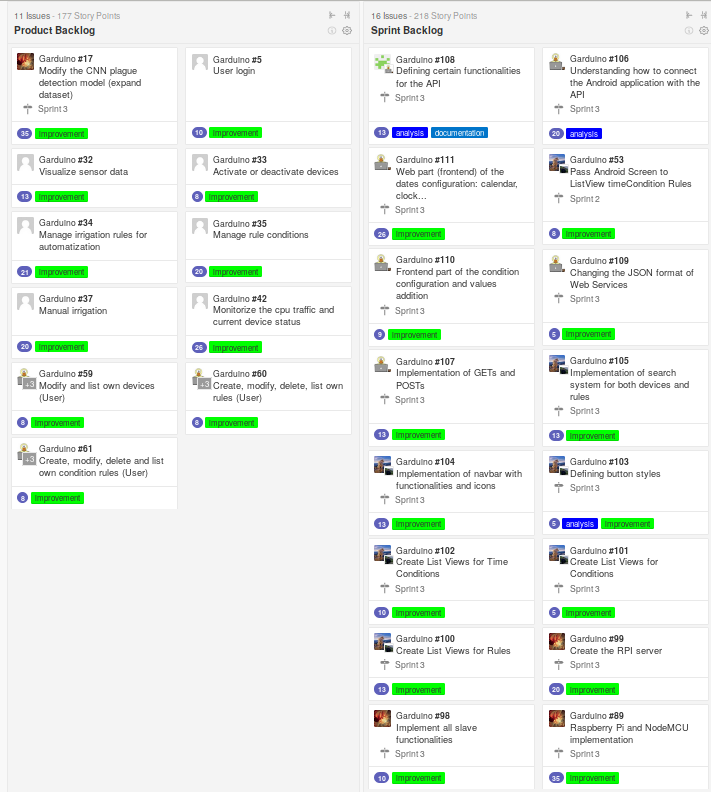
\includegraphics[scale=0.6]{Sprint3.png}
\caption{Product backlog and sprint backlog issues}
\end{figure}
\newpage
%% \section{Sprint backlog + dedication to each one}
%% Sprint backlog + dedication to each one
\begin{table}[htbp]
\begin{tabular}{|l|l|l|l|} 
\hline
Event                                                & Trigger     & Priority & Weight \\ \hline \hline
Modify the CNN plague detection model (expand dataset) & Users       & LOW     & 35  \\ \hline
User Login                                             & Users       & LOW   & 10  \\ \hline              
Visualize sensor data                                & Users/Admin & MEDIUM   & 13     \\ \hline
Enable or disable devices                            & Users       & MEDIUM   & 8      \\ \hline
Manage irrigation rules for automatization           & Users       & HIGH   & 21      \\ \hline
Manage rule conditions                               & Users       & HIGH   & 20     \\ \hline
Visualize users info                                 & Admin       & LOW      & 10     \\ \hline
Manual irrigation                                    & Users       & MEDIUM   & 20     \\ \hline
Show plaged detection analysis results               & Users       & MEDIUM   & 10     \\ \hline
Monitorize the cpu traffic and current device status & Admin       & MEDIUM   & 26     \\ \hline
Modify and list own devices                          & User        & MEDIUM   & 8      \\ \hline
Create, modify, delete, list own rules               & User        & MEDIUM   & 8      \\ \hline
Create, modify, delete, list own condition rules     & User        & MEDIUM   & 8      \\ \hline
\end{tabular}
\caption{Product Backlog explicit table}
\end{table}
The following issues have been added to the Product Backlog for the Sprint 3: 
\begin{itemize}
    \item Create, modify, delete, list own devices
    \item Create, modify, delete, list own rules
    \item Create, modify, delete, list own condition rules
\end{itemize}
\begin{table}[htbp]
\begin{tabular}{|l|l|l|l|} 
\hline
Event                                                & Trigger     & Priority & Weight \\ \hline \hline
Software Installation                                & Users       & HIGH     & 10     \\ \hline
Configure DataSource                                 & Users       & MEDIUM   & 10     \\ \hline
Define Operations Api Rest                           & Users       & LOW      & 10     \\ \hline
Api Rest Implementation                              & Users/Admin & MEDIUM   & 26     \\ \hline
Implement DataBase Class                             & Users       & MEDIUM   & 8      \\ \hline
Configure WildFly to JBOSS                           & Users       & MEDIUM   & 2      \\ \hline
Create DB Schema and Tables                          & Users       & MEDIUM   & 20     \\ \hline
Arduino Budget Analysis                              & Admin       & LOW      & 10     \\ \hline
Pop Up Screens Android                               & Users       & MEDIUM   & 20     \\ \hline
Pass Android Screen TimeConditionRules to ListView   & Users       & MEDIUM   & 10     \\ \hline
Create, modify, delete, list users                   & Admin       & MEDIUM   & 5      \\ \hline
Create, modify, delete, list devices                 & Admin       & MEDIUM   & 5      \\ \hline
Frontend screens and functionalities                 & Admin       & MEDIUM   & 5      \\ \hline
Create, modify, delete, list rules                   & Admin       & MEDIUM   & 5      \\ \hline
Create, modify, delete, list condition rules         & Admin       & MEDIUM   & 5      \\ \hline
Documentation Sprint 3                               & Team        & HIGH     & 21     \\ \hline
Prepare the slides and the presentation              & Team        & HIGH     & 8      \\ \hline
\end{tabular}
\caption{Sprint 3 Backlog explicit table}
\end{table}

\newpage
\section{Requirements}
\subsection{Non-functional requirements}
\begin{enumerate}
\item \textbf{Product}
	\begin{enumerate}
	
	\item \textbf{Accessibility and Usability}
		\begin{enumerate}
		\item Regardless of the style of interaction, the interface has to be simple and intuitive, providing a high level of interactivity and usability. The tasks will be as visual as possible, since the application will be oriented to all types of age ranges. 
		\end{enumerate}
	\item \textbf{Concurrency}
		\begin{enumerate}
		\item  The app has to be multi-user, allowing the usage of several users simultaneously of the application.
		\end{enumerate}
		
	\item \textbf{Portability}
		\begin{enumerate}
		\item \textbf{Adaptability (multi-device):} It is required that the design is "responsive" in order to ensure proper display on multiple devices, such as tablets, smartphones...
		\end{enumerate}
		
	\item \textbf{Support}
		\begin{enumerate}
		\item The mobile app will be developed by the Android platform.
		\end{enumerate}
	\end{enumerate}

\item \textbf{External}
	\begin{enumerate}
	\item \textbf{Privacy} 
		\begin{enumerate}
		\item All data management has to conform to the requirements of the organic law of data protection in order to preserve privacy in the processing of personal data.
		\end{enumerate}
		
	\end{enumerate}

\end{enumerate}

\subsection{Functional requirements}
\subsection{List of functionalities and features}
\textit{List of functionalities and features that all services (Android app, web service and Arduino) will accomplish}

\subsubsection{Android app}
\begin{itemize}
\item \textbf{The Android app will have to} allow communication with the web service.

\item \textbf{The Android app will have to} allow each user to log in.

\item \textbf{The Android app will have to} allow each user to configure/create an irrigation unit independently.

\item \textbf{The Android app will have to} show all irrigation units configured by the user.

\item \textbf{The Android app will have to} allow the manual watering option for each watering unit.

\item \textbf{The Android app will have to} allow planned irrigation of each irrigation unit.

\item \textbf{The Android app will have to} allow the option of monitoring the crop with data obtained from sensors and the webcam.

\item \textbf{The Android app will have to} allow the change of language.
\end{itemize}

\subsubsection{Web service}
\begin{itemize}
\item \textbf{The web service will have to} allow communication with the Android application and the Arduino devices.

\item \textbf{The web service will have to} allow the execution of a cron to make requests to the Arduino every X time so that a user can automatically receive notifications of his crop.

\item \textbf{The web service will have to} allow the execution of a machine learning script in charge of pest detection and return the data back to the Android application.

\item \textbf{The web service will have to} be able to determine when watering is optimal (if the automatic watering function has been used without programming) and send the request to the Arduino.

\item \textbf{The web service will have to} allow CRUD operations directly from the DB.
\end{itemize}

\subsubsection{Detection plague script}
\begin{itemize}

\item \textbf{The pest detection algorithm will have to}, using an image of a leaf as an input, determine if this is a pest or not.
\end{itemize}

\subsubsection{Arduino}
\begin{itemize}
\item \textbf{The Arduino system will have to} allow communication with the web service.

\item \textbf{The Arduino system will have to} allow images to be sent in real time to the web service.

\item \textbf{The Arduino system will have to} allow the data from the humidity, temperature and soil sensors to be captured.

\end{itemize}
\vspace{1cm}
\textit{The leaf trimming algorithm requirement has been removed because the system will have a model that will already have the capabilities to process the whole image of the plant without the need of trimming it.} 

\newpage

\section{Main use cases}
\begin{figure}[hbtp]
\centering
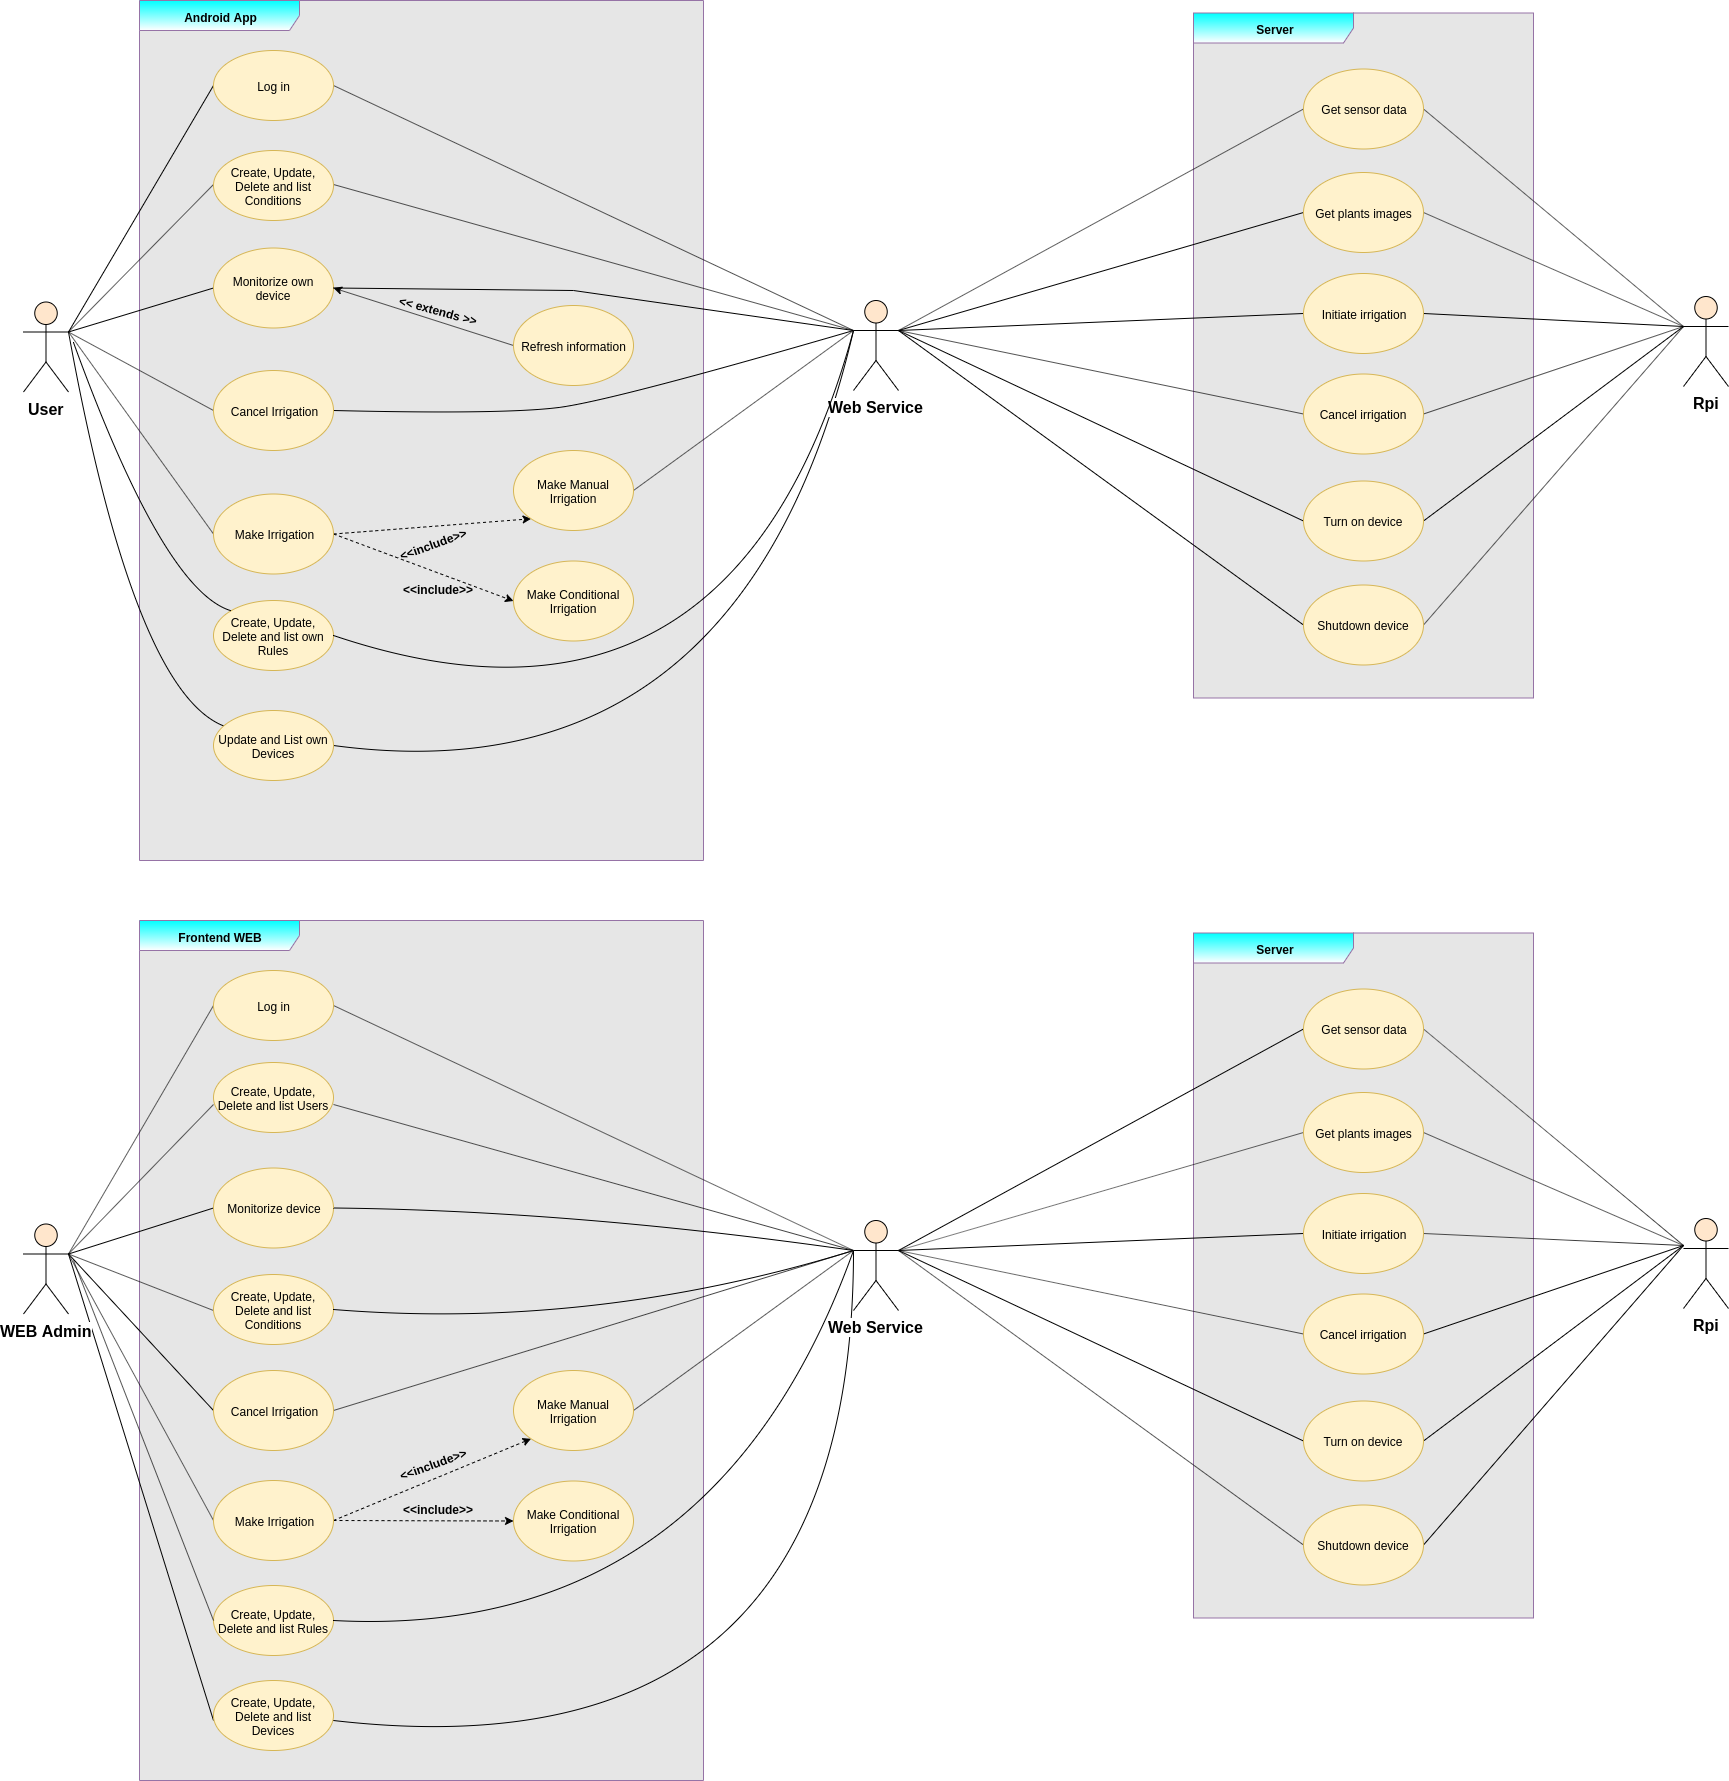
\includegraphics[scale=0.300,angle=0,origin=c]{DCU.png}
\caption{Application use cases diagram}
\label{figure2}
\end{figure} \newpage\leavevmode \\
En la \textcolor{blue}{Figure \ref{figure2}}, se muestran los siguientes actores: el usuario, el web service, el Rpi y el Admin.\newline\newline
El usuario podrá loggearse, pedir que se muestren sus instalaciones y editarlas. Además, también podrá monitorizar sus propias instalaciones. Asimismo, podrá crear, modificar, eliminar y listar tanto sus reglas como condiciones de riego. Con el objetivo de regar, el usuario podrá regar sus instalaciones manualmente y con condiciones de riego. Todas estas funcionalidades son recibidas por el Web Service el cual esperará las peticiones que se hagan desde la aplicación Android y este pedirá la información necesaria a la Rpi para poder dar dicha información a la parte Android y en consecuencia mostrarla. \newline\newline
El admin podrá loggearse, pedir que se muestren todas las instalaciones así como crearlas, modificarlas y eliminarlas. Además, también podrá monitorizarlas. A continuación, podrá crear, modificar, eliminar y listar todas las reglas, condiciones de riego y usuarios. Con el objetivo de regar, el admin podrá regar todas las instalaciones manualmente y con condiciones de riego. Todas estas funcionalidades son recibidas por el Web Service el cual esperará las peticiones que se hagan desde el frontend de la parte web y éste pedirá la información necesaria a la Rpi para poder dar dicha información a la parte del frontend y en consecuencia mostrarla.   
\newline\newline
En relación al Sprint anterior, hemos decidido cambiar la parte de Arduino por la de Rpi porque al arduino tendríamos que conectar muchos componentes // TO DO
\newpage

\section{General architecture}
\subsection{System architecture}
\begin{figure}[hbtp]
\centering
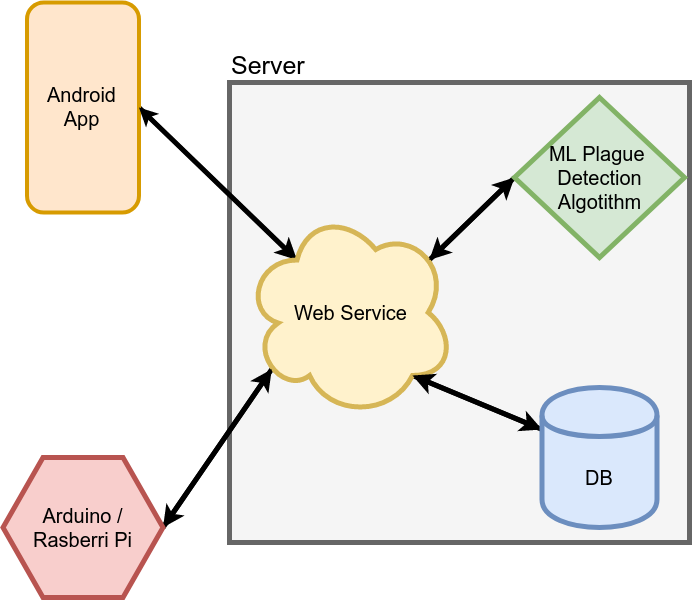
\includegraphics[scale=0.6]{AppArchitecture.png}
\caption{System app architecture}
\end{figure}

The architecture of our application is composed by:
\begin{itemize}
\item \textbf{Android App}: Graphical interface, in charge of collecting the data entered by the user.
\item \textbf{Web Service}: Makes middleware of the application. It manages requests between the Android app and the Arduino/Raspberry pi, the database, ...
\item \textbf{Arduino/Raspberry pi}: Device that will be in charge of the irrigation of each environment (gardening, flowerpot, ...).
\item \textbf{Database}: Manage all the data of the application, user credentials, register all requests, device info, ...
\end{itemize}

\newpage

\subsection{Arduino/Raspberry pi architecture}
\vspace*{3cm}
\begin{figure}[hbtp]
\centering
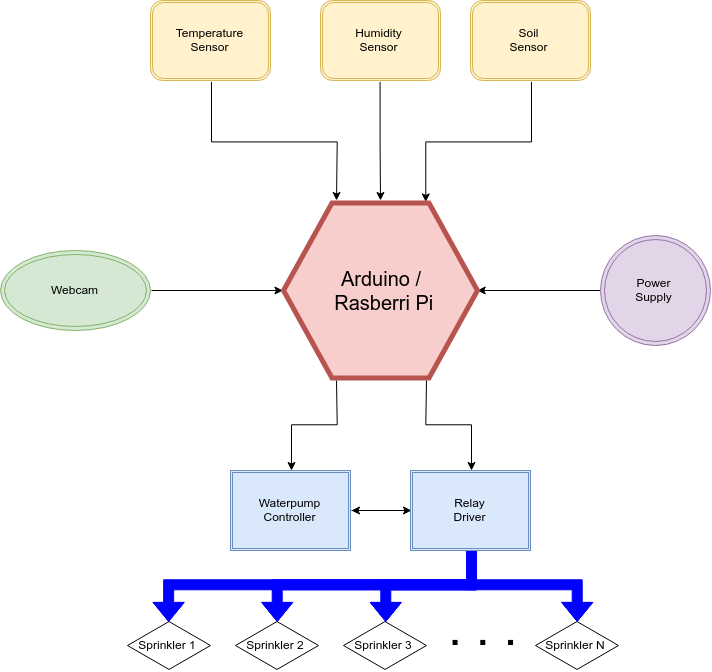
\includegraphics[scale=0.6]{ArduinoArch.png}
\caption{Arduino and rapsberry pi architecture}
\end{figure}

\newpage

\section{Data model}
%% Data model
\begin{figure}[hbtp]
\centering
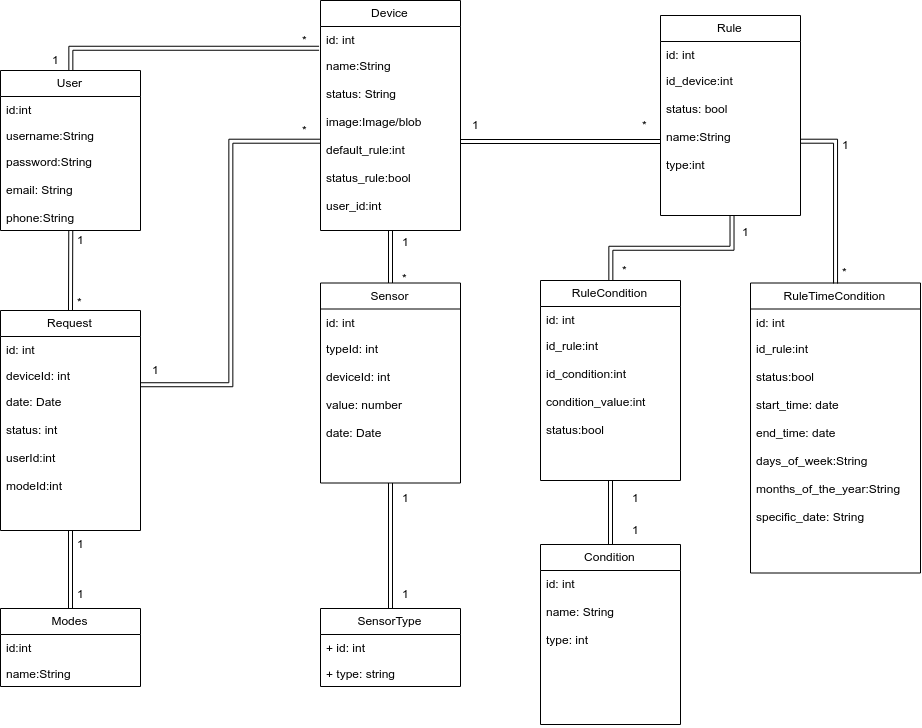
\includegraphics[scale=0.5]{ModelDeDades.png}
\caption{Data model UML}
\end{figure}
In this data model diagram we can see how our data is structured and related with the different datatables. We explain the target of the different tables:

\begin{itemize}
\item \textbf{User}: It stores all the data related to our users.

\item \textbf{Request}: It is used to store the requests of the users  to a specific device and to check if these requests have been completed. 

\item \textbf{Mode}: It stores the different kind of requests that a user can do  like manual irrigations, conditional irrigations, the obtainment of the sensor data.

\item \textbf{Device}: It stores the information of a device which corresponds to a user. It can have a default rule, so the user has not need to create its own. 

\item \textbf{Sensor}: It stores the value of a sensor of a specific type which correspond to a device.

\item \textbf{SensorType}: It stores the different type of sensors which are: Humidity, Temperature, Soil.

\item \textbf{Rule}: It stores all the configurations which correspond to a device. It can have RuleConditions and TimeConditions.

\item \textbf{RuleCondition}: It stores the conditions  with its respective value. It corresponds to a rule and a condition. If the sensors data of a device accomplish these conditions then an irrigation is produced.  

\item \textbf{RuleTimeCondition}: It corresponds to the conditions of a rule which a user decides when an irrigation has to be produced.  With the status we determine if this condition has to be considered.

\item \textbf{Condition}: It stores the different conditions which are: Temperature is lower than,Temperature is greater than, Humidity is lower than,  Humidity is greater than, Soil is lower than, Soil is greater than.
\end{itemize}

\newpage

\section{Main screens desgin and Navigation}
%% Navigation schema between activities
\begin{itemize}
\item Link Android Design:\newline\newline \textcolor{blue}{\href{https://drive.google.com/file/d/1GWvJHmUxLQVg-ns894TZreQi0Cy9rv79/view?usp=sharing}{Click here: Android Screens Navigation}}

\item Brief explanation of the different screens in the Android application: 
\\ \\Introducció
On screen 1, a list of the different devices available in the user's installation is shown. You can see the last photograph taken by the system, as well as the last date and time of irrigation. As such, the user can activate and deactivate the system for that particular device by means of a switch, or enter the panel of that particular device by pressing on the rest of the box pertinent to that device. 
\\ \\
Screen 2 shows the control panel for a particular device. The last image obtained by the system, temperature, humidity and soil can be consulted. 
You can see the last time and date the data was updated. A manual irrigation can be started and the configuration of the device can be accessed.
\\ \\
Screen 3 shows the pop-up relevant to the operation of a manual irrigation. You can enter a numerical amount on how long the irrigation will last, and you are given the option of initializing the irrigation or canceling it.
\\ \\
Screen 4 shows the control panel of a device when there is a manual irrigation in progress. It indicates how much irrigation time is left, and offers the option of cancelling it instantaneously. 
\\ \\
Screen 5 shows the configuration menu of a device. It offers the option to change its name, change the frequency of updating information and access to a panel to modify the irrigation rules. All changes will be saved when you press the save button. 
\\ \\
Screen 6 shows the configuration panel of a device's irrigation ruleset. It shows the list of rules, which can be activated and deactivated by means of a switch, and these can be modified by clicking on them. It shows the option to add new rules and the option to save changes.
\\ \\
Screen 7 shows the irrigation rule creation screen. You can choose its name, confirm its creation and cancel it. This screen will be converted to a pop-up in the near future of the development of the project. 
\\ \\
Screen 8 shows the configuration panel of the irrigation rules of a device after a new irrigation rule has been created. The internal configuration of this can now be accessed and modified by clicking on its name. 
\\ \\
Screen 9 shows the configuration panel of an irrigation rule. This will consist of various conditions, which can be activated and deactivated through the use of a switch. It offers the option to modify the parameters of the conditions, as well as to create a new one and save the changes in that irrigation rule. 
\\ \\
Screen 10 shows the screen to add a new condition. It shows the different types of conditions that are available. 
\\ \\
Screen 11 shows the configuration of a time condition. It shows the various options for which the condition will be active: start and end time of the days it will be active, configuration by days of the week, by months in which it will be active, and specific dates in which the time condition will be active. 
\\ \\
Screen 12 shows the modification of one of the parameters related to the time of a time condition (start time and end time). The specific times can be selected by specifying them in a clock. 
\\ \\
Screen 13 shows the modification of the parameters relative to the specific dates in which the time condition will operate. The specific days can be chosen by means of a calendar. 
\\ \\
As an improvement of the previous prototype, some screens have been changed by the pop-ups corresponding to these in order to streamline navigation and maintain an awareness of the location between the various screens on which the user navigates at all times. 

\item Link Web Design:
\end{itemize}
\section{Financial Factors}
\section{Economic viability}
\subsection{Who?}
The customer profile should be the one interested in controlling the irrigation and the health of the plants in your house in a comfortable, efficient and automated way. The population segment defined as target audience is broad and determined by these very simple conditions. \\

It can be focused both on private gardening and on a larger scale. Volume limits are set by the customer's business model or personal use. \\

Likewise, the company bets on the provision to distributors and garden shops, as well as the direct provision to individuals.\\

It will begin marketing the product in the area of Catalonia, where it will be made known to local distributors and will provide support in installation, configuration and maintenance to customers. 
\subsection{How many?}
An incremental and exponential progress of the user base is estimated as a function of the increase in the company's resources as a result of the successful marketing and expansion of the product. As such, it is estimated that some representative figures of success in the first year are: 

\begin{itemize}
\item To have marketed and installed and to have in maintenance 100 devices in particular. 
\item To have established supply agreements with 2 distributors. 
\end{itemize}
A significant potential progression would be:
\begin{table}[htbp]
\centering
\begin{tabular}{|l|l|l|l|l|l|}
\hline
\textbf{} & \textbf{Year 1} & \textbf{Year 2} & \textbf{Year 3} & \textbf{Year 4} & \textbf{Year 5} \\
\hline \hline
Particularities & 100 & 250 & 500 & 1000 & 2000 \\
\hline
Distributors & 2 & 4 & 6 & 8 & 10 \\
\hline
\end{tabular}
\caption{Table of potential marketing progression}
\end{table}

\subsection{Mareketing strategy}
The main comunication Garduino objectives are:
\begin{itemize}
\item Promote the notoriety of the brand and/or product marketed among the target audience.
\item Promote knowledge of product attributes, characteristics and performance, as well as competitive differentiation with respect to the same product market.
\item Establish and strengthen a connection between company and target audience, carrying out different strategies to familiarize and bring the user closer to the brand and product in marketing.
\item To constitute, with regard to the potential client, one of the alternatives of the market to contemplate when acquiring a product of the nature of the article in question.
\end{itemize}

The public of interest is understood to be the group of publics or audiences targeted by a marketing campaign. It should be noted that we can differentiate between primary and secondary audiences, depending on whether or not they are involved as potential end consumers.\\

As such, it has established a profile of primary interest audience of the characteristics described in the section "Who"?\\ 

The communication techniques used for the promotion and diffusion of brand and product will be the following:\\
\begin{itemize}
\item \textbf{Advertising in conventional media}: transmission of the advertising message through advertisements and programmed messages in media such as television, radio...
\item \textbf{Sales promotion}: alterations in the sales lot or in the price of the product in order to attract consumers.
\item \textbf{Fairs and exhibitions}: Participation and presence in fairs and exhibitions to make oneself known or to collaborate in the transmission of a message. 
\item \textbf{Sponsorship}: Association with other initiatives, businesses, causes and figures in order to carry out an exhibition of the brand in certain contexts, as well as to carry out an exploitation of the image associated with the activity in question, and to try to carry out a commercial exploitation of activities derived from the event.
\item \textbf{Personal sale}: Presential presentation and sale of the commercial to the client of the product in a physical space. This technique is usually carried out in commercial spaces, by means of informative and/or exhibition stands where the product is presented to the client and it is a question of negotiating a closing of sales with the same one. 
\item \textbf{Website}: Use of an informative web space where relevant company information can be announced, as well as support for online sales and subscription to other types of digital communications.
\item \textbf{Blogs}: Use of web spaces structured through a system of publication of articles and news over time, which can allow different degrees of participation by users, and through which it is intended to capture an interest in the user and redirect traffic to the main website or digital content that presents information on products that may be of interest to the potential consumer.
\item \textbf{Social networks}: Use of social network platforms to maintain a system of communication and promotion with the user, in addition to being a powerful tool for the approach and contact with it.
\item \textbf{E-mailing}: newsletter system that transmits information and advertising relevant to the brand and product through e-mail. 
\end{itemize}
\vspace{0.6in}
The communication model presented by Garduino is the multiphase model. This communication model not only involves commercials and experts or opinion leaders as influential and diffusion figures, but it will be the target public itself that will assume a role of active participation within the communicative process. These will act as "ambassadors" of a product, brand, good, service...\\ 

\newpage

This model manifests itself strongly in the growing digital and social network environments, and the search for the implementation of this kind of model by companies is evident in the incitement for the user to participate in one of the dissemination campaigns through these environments. It is also considered that this strategy will be based on the principles of inbound marketing:\\
\begin{figure}[hbtp]
\centering
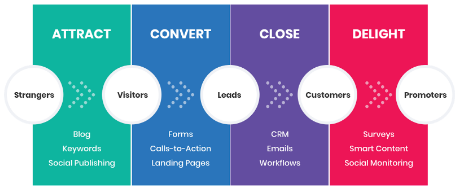
\includegraphics[scale=1]{marketing.png}
\caption{Inbound marketing scheme}
\end{figure}

\subsection{Monetization strategy}
The main sources of revenue for the business model will be: 
\begin{itemize}
\item Sale of the software to individuals
\item Sale of the software to distributors
\item Sale of the devices to private individuals
\item Sale of devices to suppliers
\item Installation service
\item Maintenance service
\item Special customization service
\end{itemize}

\subsection{App costs}
\begin{itemize}
\item \textbf{App type}: app for the management and monitoring of irrigation and pest control installations. 
\item \textbf{App platform}: Android (potentially IOS, in the future)
Coding: The start-up partners will act as developers of the project software. 
\item \textbf{Features}: Configuration of the installed devices, live monitoring, notification system for events such as detection of anomalies/pests...
\item \textbf{UI Design \& Graphics}: The interface design of the app must be intuitive and user-friendly, while covering a high degree of customization options for irrigation systems. 
\item \textbf{Marketing}: The stipulated communication campaign will be followed, whose investment will be proportional to the level of income generated at each moment of the life phase of the product. 
\item \textbf{Operational costs}: Costs for the Arduino parts of the prototypes, electricity costs and maintenance of the computers with which the project is programmed. 
\end{itemize}

\subsection{Analysis}
\begin{table}[htbp]
\centering
\begin{tabular}{|l||l|l|l|l|l|}
\hline
\textbf{} & \textbf{Year 1} & \textbf{Year 2} & \textbf{Year 3} & \textbf{Year 4} & \textbf{Year 5} \\ \hline \hline
Income & 20.000\euro{} & 50.000\euro{} & 100.000\euro{} & 200.000\euro{} & 400.000\euro{} \\ \hline
Expenses & 35.000\euro{} & 65.000\euro{} & 65.000\euro{} & 115.000\euro{} & 215.000\euro{} \\ \hline
Benefit & -15.000\euro{} & -15.000\euro{} & 35.000\euro{} & 85.000\euro{} & 185.000\euro{} \\ \hline
\end{tabular}
\caption{Table of economic analysis}
\end{table}

\end{document}

